% -*- Mode: latex; -*-
% $HeadURL$
% $Id$


\HPCToolkit{} provides the \hpcviewer{}~\cite{Adhianto-MC-Ta:2010:PSTI-hpcviewer} performance presentation tool for interactive examination of performance databases.
\hpcviewer{} interactively presents context-sensitive performance metrics correlated to program structure and mapped to a program's source code, if available.
It can present an arbitrary collection of performance metrics gathered during one or more runs or compute derived metrics.


% ===========================================================================
% ===========================================================================

\section{Launching}

\hpcviewer{} can either be launched from a command line (Linux/Unix platform) or by clicking the \hpcviewer{} icon (for Windows, Mac OS X and Linux/Unix platform).
The command line syntax is as follows:
\begin{quote}
\begin{verbatim}
  hpcviewer [options] [<hpctoolkit-database>]
\end{verbatim}
\end{quote}
Here, \texttt{<hpctoolkit-database>} is an optional argument to load a database automatically.
Without this argument, \hpcviewer{} will prompt for the location of a database.

The possible options are as follows:
\begin{itemize}
 \item \texttt{-n}: Do not display the Callers View.  (Saves memory and time.)

 \item \texttt{-consolelog}: Send log entries to a console in addition to a log file.
   (To get a console window, be sure to use java as the VM instead of javaw.)

 \item \texttt{-debug}: Log additional information about plug-in dependency problems.
\end{itemize}


% ===========================================================================
% ===========================================================================

\begin{comment}
\section{Installing \hpcviewer{}}

\subsection{Requirements}
\begin{itemize}
 \item Java Runtime Environment (JRE) 1.5 or greater.
   Use the Oracle or IBM version; we have had problems with OpenJDK.
   Specifically we recommend Oracle on x86 platforms, and IBM java on POWER.
   Take special note on POWER systems: we require the 64-bit java, even on a 32-bit
   platform.

 \item On Linux, GTK+ is required.
\end{itemize}


\subsection{Generic Instructions}
\begin{enumerate}
  \item Download \hpcviewer{} package that is suitable for your platform from 
    \begin{quote}
      \url{https://outreach.scidac.gov/frs/?group\_id=22} 
    \end{quote}
  \item Untar the tarball into a temporary directory (Linux) or an installation directory (Windows and Mac).
\end{enumerate}


\subsection{Linux-specific Instructions}

To install \hpcviewer{} in an \HPCToolkit{} installation, unpack the tarball and execute the following command:
\begin{quote}
\begin{verbatim}
  ./<hpcviewer>/install [-j <path-to-java>] <install-path>
\end{verbatim}
\end{quote}
Here, \mytt{<hpcviewer>} is the directory created by unpacking the tarball; and 
\mytt{<install-path>} is the same directory passed to the \texttt{--prefix} option of \HPCToolkit{}'s \texttt{configure} script.
The optional \mytt{-j} flag configures the java to be used with \mytt{<hpcviewer>}. If the \mytt{-j} flag is unspecified,
then the java found on the path will be used.

Typically one compiles and installs \HPCToolkit{} before installing \hpcviewer{}, but this is not necessary.
Note, however, that if \hpcviewer{} is installed first, the \mytt{install} script will issue a warning and request confirmation.
\end{comment}

% ===========================================================================
% ===========================================================================

\section{Views}

\begin{figure}[t]
\centering{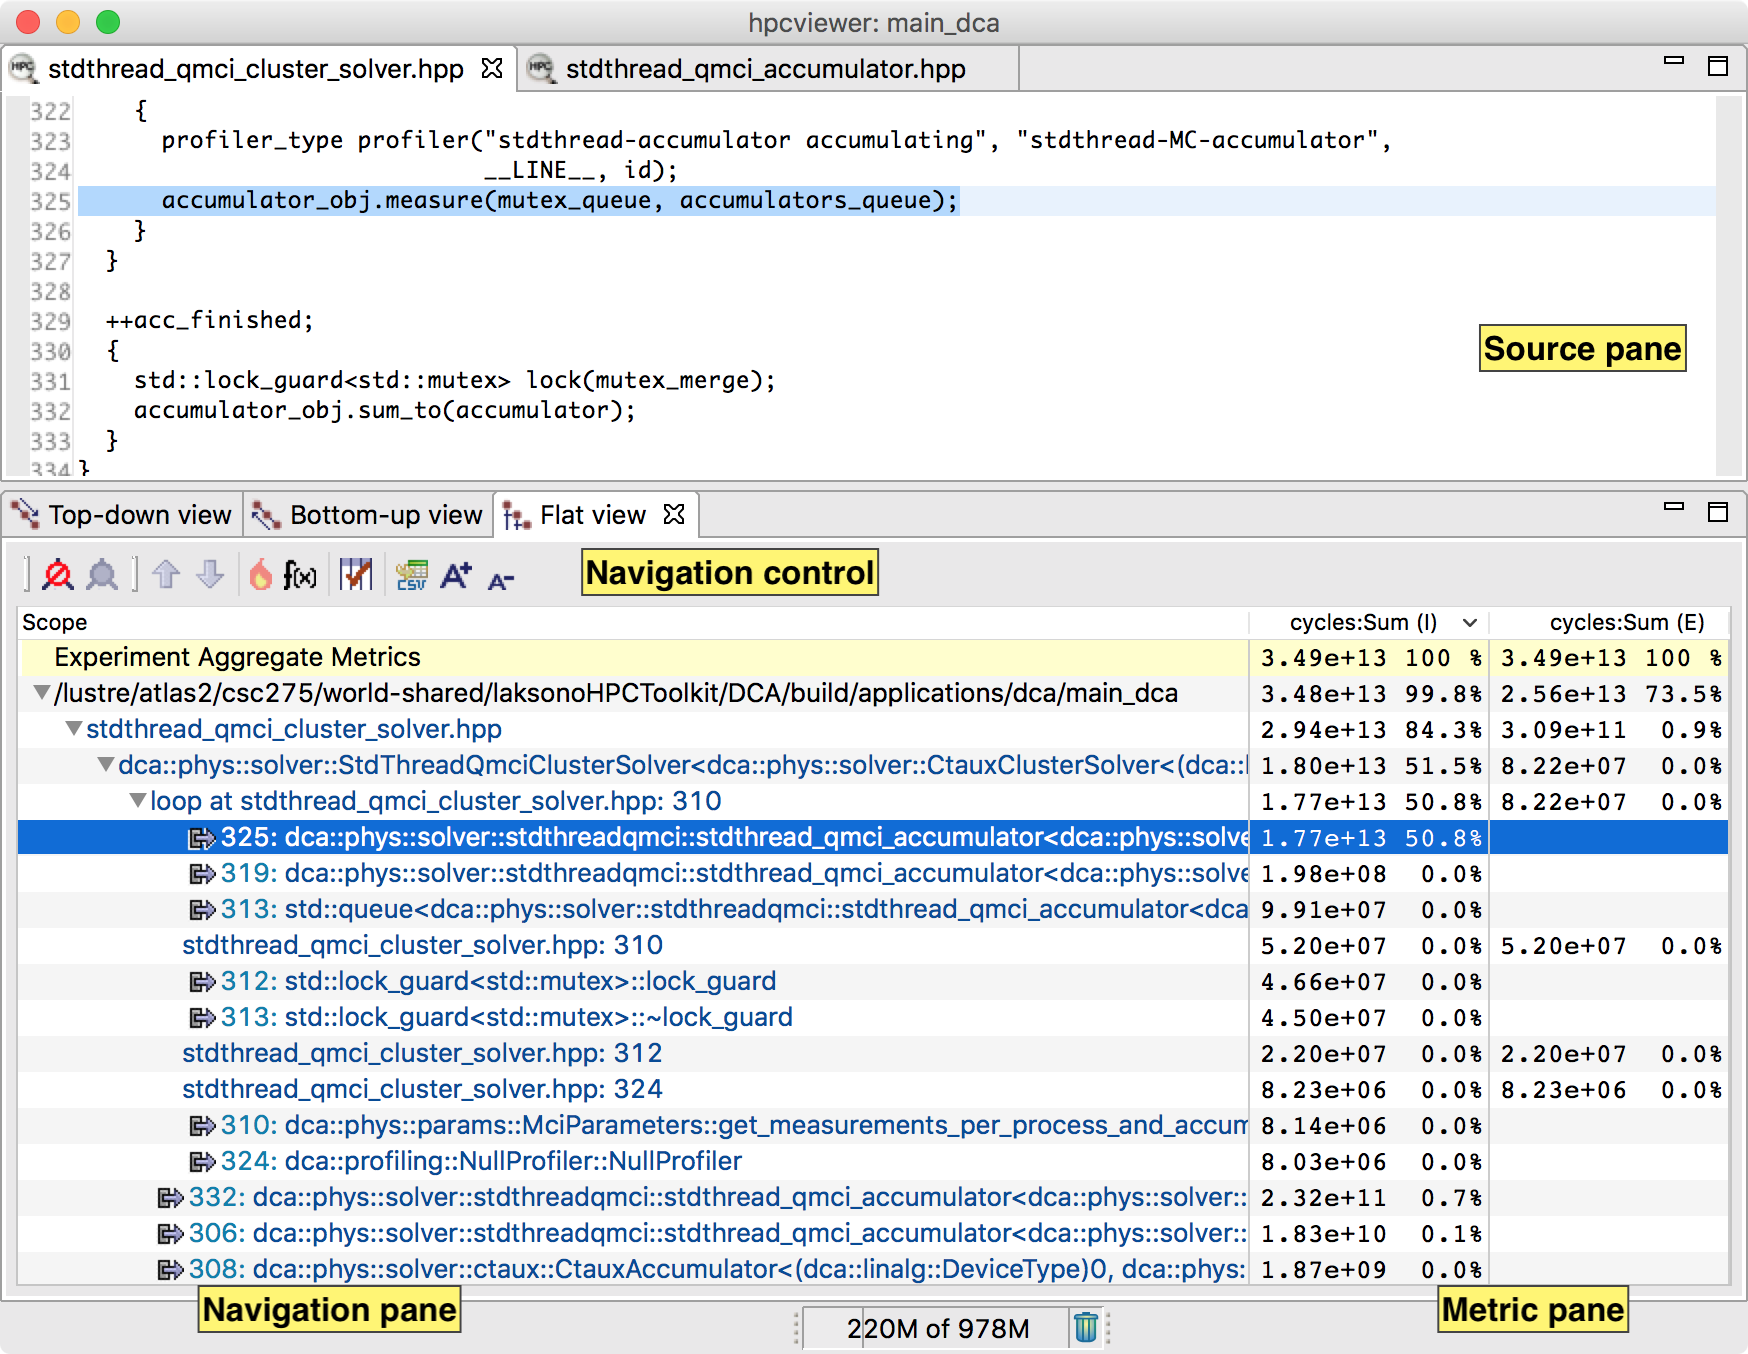
\includegraphics[width=\textwidth]{fig/hpcviewer-legend.png}}
\caption{An annotated screenshot of \hpcviewer{}'s interface.}
\label{fig:hpcviewer-legend}
\end{figure}

Figure~\ref{fig:hpcviewer-legend} shows an annotated screenshot of \hpcviewer{}'s user interface presenting a call path profile.
The annotations highlight \hpcviewer{}'s principal window panes and key controls.
The browser window is divided into three panes.
The Source pane (top) displays program source code.
The Navigation and Metric panes (bottom) associate a table of performance metrics with static or dynamic program structure.
These panes are discussed in more detail in Section~\ref{sec:hpcviewer:panes}.

\hpcviewer{} displays calling-context-sensitive performance data in three different views: a top-down \emph{Calling Context View}, a bottom-up \emph{Callers View}, and a \emph{Flat View}.
One selects the desired view by clicking on the corresponding view control tab.
We briefly describe the three views and their corresponding purposes.

\begin{itemize}
\item \textbf{Calling Context View}.
  This top-down view represents the dynamic calling contexts (call paths) in which costs were incurred.
  Using this view, one can explore performance measurements of an application in a top-down fashion to understand the costs incurred by calls to a procedure in a particular calling context.
  We use the term \emph{cost} rather than simply \emph{time} since \hpcviewer{} can present a multiplicity of measured such as cycles, or cache misses) or derived metrics (\eg{} cache miss rates or bandwidth consumed) that that are other indicators of execution cost.

  A calling context for a procedure \fnnm{f} consists of the stack of procedure frames active when the call was made to \fnnm{f}.
  Using this view, one can readily see how much of the application's cost was incurred by \fnnm{f} when called from a particular calling context.
  If finer detail is of interest, one can explore how the costs incurred by a call to \fnnm{f} in a particular context are divided between \fnnm{f} itself and the procedures it calls.
  \HPCToolkit{}'s call path profiler \hpcrun{} and the \hpcviewer{} user interface distinguish calling context precisely by individual call sites; this means that if a procedure \fnnm{g} contains calls to procedure \fnnm{f} in different places, these represent separate calling contexts.

\item \textbf{Callers View}.
  This bottom-up view enables one to look upward along call paths.
  The view apportions a procedure's costs to its caller and, more generally, its calling contexts.
  This view is particularly useful for understanding the performance of software components or procedures that are used in more than one context.
  For instance, a message-passing program may call \mytt{MPI_Wait} in many different calling contexts.
  The cost of any particular call will depend upon the structure of the parallelization in which the call is made.
  Serialization or load imbalance may cause long waits in some calling contexts while other parts of the program may have short waits because computation is balanced and communication is overlapped with computation.

  When several levels of the Callers View are expanded, saying that the Callers View apportions metrics of a callee on behalf of its caller can be confusing: what is the caller and what is the callee?
  In this situation, we can say that the Callers View apportions the metrics of a particular procedure \emph{in its various calling contexts} on behalf of that context's caller.
  Alternatively but equivalently, the Callers View apportions the metrics of a particular procedure on behalf of its various \emph{calling contexts}.

\item \textbf{Flat View}.
  This view organizes performance measurement data according to the static structure of an application.
  All costs incurred in any calling context by a procedure are aggregated together in the Flat View.
  This complements the Calling Context View, in which the costs incurred by a particular procedure are represented separately for each call to the procedure from a different calling context.

\end{itemize}


% ===========================================================================
% ===========================================================================

\section{Panes}
\label{sec:hpcviewer:panes}

\hpcviewer{}'s browser window is divided into three panes: the \emph{Navigation pane}, \emph{Source pane}, and the \emph{Metrics pane}.
We briefly describe the role of each pane.

% ==========================================================
% ==========================================================

\subsection{Source pane}
\label{sec:pane-source}

The source pane displays the source code associated with the current entity selected in the navigation pane.
When a performance database is first opened with \hpcviewer{}, the source pane is initially blank because no entity has been selected in the navigation pane.
Selecting any entity in the navigation pane will cause the source pane to load the corresponding file, scroll to and highlight the line corresponding to the selection.
Switching the source pane to view to a different source file is accomplished by making another selection in the navigation pane.

% ==========================================================
% ==========================================================

\subsection{Navigation pane}

The navigation pane presents a hierarchical tree-based structure that is used to organize the presentation of an applications's performance data.
Entities that occur in the navigation pane's tree include load modules, files, procedures, procedure activations, inlined code, loops, and source lines.
Selecting any of these entities will cause its corresponding source code (if any) to be displayed in the source pane.
One can reveal or conceal children in this hierarchy by `opening' or `closing' any non-leaf (\ie{}, individual source line) entry in this view.

The nature of the entities in the navigation pane's tree structure depends upon whether one is exploring the Calling Context View, the Callers View, or the Flat View of the performance data.
\begin{itemize}
\item In the \textbf{Calling Context View}, entities in the navigation tree represent procedure activations, inlined code, loops, and source lines.
  While most entities link to a single location in source code, procedure activations link to two: the call site from which a procedure was called and the procedure itself.

\item In the \textbf{Callers View}, entities in the navigation tree are procedure activations.
  Unlike procedure activations in the calling context tree view in which call sites are paired with the called procedure, in the caller's view, call sites are paired with the calling procedure to facilitate attribution of costs for a called procedure to multiple different call sites and callers.

\item In the \textbf{Flat View}, entities in the navigation tree correspond to source files, procedure call sites (which are rendered the same way as procedure activations), loops, and source lines.
\end{itemize}

\subsubsection{Navigation control}

The header above the navigation pane contains some controls for the navigation and metric view.
In Figure~\ref{fig:hpcviewer-legend}, they are labeled as ``navigation/metric control.''
\begin{itemize}

\item \textbf{Flatten} 
\includegraphics[scale=.8]{fig/hpcviewer-button-flatten.png} /
      \textbf{Unflatten} 
\includegraphics[scale=.8]{fig/hpcviewer-button-unflatten.png}
      (available for the Flat View):

Enabling to flatten and unflatten the navigation hierarchy.
Clicking on the flatten button (the icon that shows a tree node with a slash through it) will replace each top-level scope shown with its children.
If a scope has no children (\ie{}, it is a leaf ), the node will remain in the view.
This flattening operation is useful for relaxing the strict hierarchical view so that peers at the same level in the tree can be viewed and ranked together.
For instance, this can be used to hide procedures in the Flat View so that outer loops can be ranked and compared to one another.
The inverse of the flatten operation is the unflatten operation, which causes an elided node in the tree to be made visible once again.

\item \textbf{Zoom-in} 
\includegraphics[scale=.8]{fig/hpcviewer-button-zoomin.png} /
      \textbf{Zoom-out} 
\includegraphics[scale=.8]{fig/hpcviewer-button-zoomout.png} :

Depressing the up arrow button will zoom in to show only information for the selected line and its descendants.
One can zoom out (reversing a prior zoom operation) by depressing the down arrow button.

\item \textbf{Hot call path} 
\includegraphics[scale=.8]{fig/hpcviewer-button-hotpath.png} :

This button is used to automatically find hot call paths with respect to the currently selected metric column.
The hot path is computed by comparing parent and child metric values, and showing the chain where the difference is greater than a threshold (by default is \texttt{50\%}).
It is also possible to change the threshold value by clicking the menu File|Preference.

\item \textbf{Derived metric} 
\includegraphics[scale=.8]{fig/hpcviewer-button-derivedmetric.png} :

Creating a new metric based on mathematical formula.
See Section~\ref{sec:hpcviewer:derived-metrics} for more details.

\item \textbf{Hide/show metrics} 
\includegraphics[scale=.8]{fig/hpcviewer-button-checkcolumns.png} :

Showing and hiding metric columns.
A dialog box will appear, and user can select which columns to show or hide.
See Section~\ref{sec:hpcviewer:metric-pane} section for more details.

\item \textbf{Export into a CSV format file} 
\includegraphics[scale=.8]{fig/hpcviewer-button-csv.png} :

Exporting the current metric table into a comma separated value (CSV) format file.
This feature only exports all metrics that are currently shown.
Metrics that are not shown in the view (whose scopes are not expanded) will not be exported (we assume these metrics are not significant).

\item \textbf{Increase font size} 
\includegraphics[scale=.8]{fig/hpcviewer-button-fontplus.png} /
      \textbf{Decrease font size} 
\includegraphics[scale=.8]{fig/hpcviewer-button-fontminus.png} :

Increasing or decreasing the size of the navigation and metric panes.

\item \textbf{Showing graph of metric values} 
\includegraphics[scale=.8]{fig/hpcviewer-button-graph.png} :

Showing the graph (plot, sorted plot or histogram) of metric values of the selected node in CCT for all processes or threads (Section~\ref{sec:hpcviewer:plots}). This menu is only available if the database is generated by \texttt{hpcprof-mpi} instead of \texttt{hpcprof}. 

\end{itemize}


\subsubsection{Context menus}
\begin{figure}
\centering{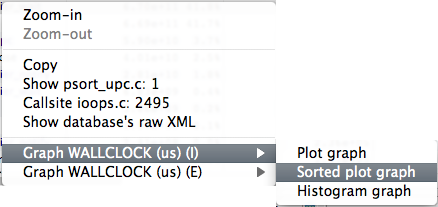
\includegraphics[width=3in]{fig/hpcviewer-menu-context-sensitive.png}}
\caption{Context menu in the navigation pane: activated by clicking the right-button of the mouse.}
\label{fig:hpcviewer-menu-context}
\end{figure}
Navigation control also provides several context menus by clicking the right-button of the mouse. As shown in Figure~\ref{fig:hpcviewer-menu-context}, the menus are:
\begin{itemize}
 \item \textbf{Zoom-in/out}: Carrying out exactly the same as action as the Zoom-in/out in the navigation control.
 \item \textbf{Copy}: Copying into clipboard the selected line in navigation pane which includes the name of the node in the tree, and the values of visible metrics in metric pane (Section ~\ref{sec:pane-metric}). The values of hidden metrics will not be copied.
 \item \textbf{Show ...}: Showing the source code file and highlighting the specified line in (Section Source pane~\ref{sec:pane-source}). If the file doesn't exist, the menu is disabled.
 \item \textbf{Callsite ...}: Showing the source code file and highlighting the specified line of the call site. This menu only available in Calling Context View. If the file doesn't exist, the menu is disabled.
 \item \textbf{Graph ...}: Showing the graph (plot, sorted plot or histogram) of metric values of the selected node in CCT for all processes or threads (Section~\ref{sec:hpcviewer:plots}). This menu is only available if the database is generated by \texttt{hpcprof-mpi} instead of \texttt{hpcprof}. 
\end{itemize}


% ==========================================================
% ==========================================================

\subsection{Metric pane}
\label{sec:pane-metric}

The metric pane displays one or more performance metrics associated with entities to the left in the navigation pane.
Entities in the tree view of the navigation pane are sorted at each level of the hierarchy by the metric in the selected column.
When \hpcviewer{} is launched, the leftmost metric column is the default selection and the navigation pane is sorted according to the values of that metric in descending order.
One can change the selected metric by clicking on a column header.
Clicking on the header of the selected column toggles the sort order between descending and ascending.

During analysis, one often wants to consider the relationship between two metrics.
This is easier when the metrics of interest are in adjacent columns of the metric pane.
One can change the order of columns in the metric pane by selecting the column header for a metric and then dragging it left or right to its desired position.
The metric pane also includes scroll bars for horizontal scrolling (to reveal other metrics) and vertical scrolling (to reveal other scopes).
Vertical scrolling of the metric and navigation panes is synchronized.


% ===========================================================================
% ===========================================================================

\section{Understanding Metrics}

\hpcviewer{} can present an arbitrary collection of performance metrics gathered during one or more runs, or compute derived metrics expressed as formulae with existing metrics as terms.

For any given scope in \hpcviewer{}'s three views, \hpcviewer{} computes both \emph{inclusive} and \emph{exclusive} metric values.
For the moment, consider the Calling Context View.
Inclusive metrics reflect costs for the entire subtree rooted at that scope.
Exclusive metrics are of two flavors, depending on the scope.
For a procedure, exclusive metrics reflect all costs within that procedure but excluding callees.
In other words, for a procedure, costs are exclusive with respect to dynamic call chains.
For all other scopes, exclusive metrics reflect costs for the scope itself; \ie{}, costs are exclusive with respect to static structure.
The Callers and Flat Views contain inclusive and exclusive metric values that are relative to the Calling Context View.
This means, \eg{}, that inclusive metrics for a particular scope in the Callers or Flat View are with respect to that scope's subtree in the Calling Context View.


% ==========================================================
% ==========================================================

\subsection{How metrics are computed?}

Call path profile measurements collected by \hpcrun{} correspond directly to the Calling Context View.
\hpcviewer{} derives all other views from exclusive metric costs in the Calling Context View.
For the Caller View, \hpcviewer{} collects the cost of all samples in each function and attribute that to a top-level entry in the Caller View.
Under each top-level function, \hpcviewer{} can look up the call chain at all of the context in which the function is called.
For each function, \hpcviewer{} apportions its costs among each of the calling contexts in which they were incurred.
\hpcviewer{} computes the Flat View by traversing the calling context tree and attributing all costs for a scope to the scope within its static source code structure.
The Flat View presents a hierarchy of nested scopes for load modules, files, procedures, loops, inlined code and statements.


% ==========================================================
% ==========================================================

\subsection{Example}

\begin{figure}[t]
\centering{%
\begin{tabular}{|p{2.7in}|p{2.7in}|}
\hline
\textbf{file1.c} & \textbf{file2.c} \\
\hline
\begin{verbatim}
f () {
  g ();
}

// m is the main routine
m () {
  f ();
  g ();
}
\end{verbatim}%
  & %
\begin{verbatim}
// g can be a recursive function
g () {
  if ( . . ) g ();
  if ( . . ) h ();
}

h () {
}
\end{verbatim}%
  \\
\hline
\end{tabular}%
}
\caption{A sample program divided into two source files.}
\label{fig:source-files}
\end{figure}



\begin{figure}[t]
\centering{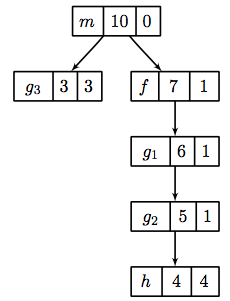
\includegraphics[scale=0.5]{fig/metrics-cct.png}}
\caption{Calling Context View. Each node of the tree has three boxes: the left-most is the name of the node (or in this case the name of the routine, the center is the inclusive value, and on the right is the exclusive value.}
\label{fig:cct}
\end{figure}

\begin{figure}
\centering{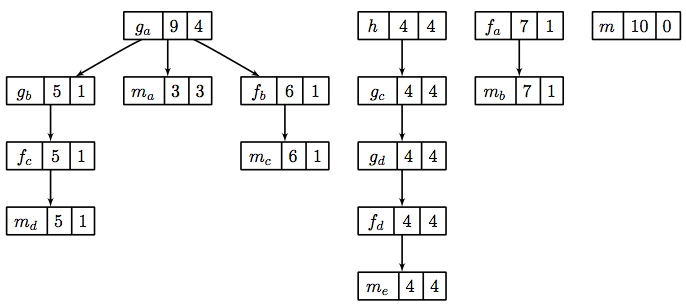
\includegraphics[scale=0.5]{fig/metrics-callers.png}}
\caption{Caller View}
\label{fig:metrics-callers}
\end{figure}

\begin{figure}
\centering{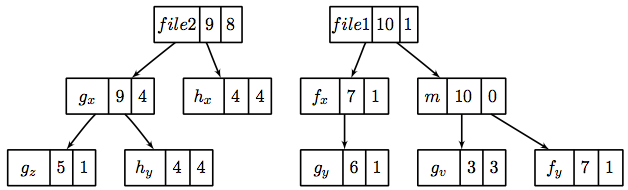
\includegraphics[scale=0.5]{fig/metrics-flat.png}}
\caption{Flat View}
\label{fig:metrics-flat}
\end{figure}


Figure~\ref{fig:source-files} shows an example of a recursive program separated into two files, \texttt{file1.c} and \texttt{file2.c}.
In this figure, we use numerical subscripts to distinguish between different instances of the same procedure.
In the other parts of this figure, we use alphabetic subscripts.
We use different labels because there is no natural one-to-one correspondence between the instances in the different views.

Routine \texttt{g} can behave as a recursive function depending on the value of the condition branch (lines 3--4).
Figure~\ref{fig:cct} shows an example of the call chain execution of the program annotated with both inclusive and exclusive costs.
Computation of inclusive costs from exclusive costs in the Calling Context View involves simply summing up all of the costs in the subtree below.

In this figure, we can see that on the right path of the routine \texttt{m}, routine \texttt{g} (instantiated in the diagram as \texttt{g$_1$}) performed a recursive call (\texttt{g$_2$}) before calling routine \texttt{h}.
Although \texttt{g$_1$}, \texttt{g$_2$} and \texttt{g$_3$} are all instances from the same routine (\ie{}, \texttt{g}), we attribute a different cost for each instance.
This separation of cost can be critical to identify which instance has a performance problem.

Figure~\ref{fig:metrics-callers} shows the corresponding scope structure for the Caller View and the costs we compute for this recursive program.
The procedure \texttt{g} noted as \texttt{g$_a$} (which is a root node in the diagram), has different cost to \texttt{g} as a callsite as noted as \texttt{g$_b$}, \texttt{g$_c$} and \texttt{g$_d$}.
For instance, on the first tree of this figure, the inclusive cost of \texttt{g$_a$} is \texttt{9}, which is the sum of the highest cost for each branch in calling context tree (Figure~\ref{fig:cct}): the inclusive cost of \texttt{g$_3$} (which is \texttt{3}) and \texttt{g$_1$} (which is \texttt{6}).
We do not attribute the cost of \texttt{g$_2$} here since it is a descendant of \texttt{g$_1$} (in other term, the cost of \texttt{g$_2$} is included in \texttt{g$_1$}).

Inclusive costs need to be computed similarly in the Flat View.
The inclusive cost of a recursive routine is the sum of the highest cost for each branch in calling context tree.
For instance, in Figure~\ref{fig:metrics-flat}, The inclusive cost of \texttt{g$_x$}, defined as the total cost of all instances of \texttt{g}, is \texttt{9}, and this is consistently the same as the cost in caller tree.
The advantage of attributing different costs for each instance of \texttt{g} is that it enables a user to identify which instance of the call to \texttt{g} is responsible for performance losses.


% ===========================================================================
% ===========================================================================

\section{Derived Metrics}
\label{sec:hpcviewer:derived-metrics}

Frequently, the data become useful only when combined with other information such as the number of instructions executed or the total number of cache accesses.
While users don't mind a bit of mental arithmetic and frequently compare values in different columns to see how they relate for a scope, doing this for many scopes is exhausting.
To address this problem, \hpcviewer{} provides a mechanism for defining metrics.
A user-defined metric is called a ``derived metric.''
A derived metric is defined by specifying a spreadsheet-like mathematical formula that refers to data in other columns in the metric table by using \texttt{\$n} to refer to the value in the \texttt{n}\textsuperscript{th} column.

% ==========================================================
% ==========================================================

\subsection{Formulae}

The formula syntax supported by \hpcviewer{} is inspired by spreadsheet-like in-fix mathematical formulae.
Operators have standard algebraic precedence.
%% The in-fix syntax is very simple, for example:
%% \begin{quote}
%% \begin{verbatim}
%% <expression>     ::= <binary_op> | <function>
%% <binary_op>      ::= <expression> <binary_operand> <expression>
%% <binary_operand> ::= + | - | * | /
%% \end{verbatim}
%% \end{quote}
%
%\paragraph{Intrinsic Functions}
%The list of intrinsic functions supported can be found in \href{functions.html}{here}.
%Creating a new intrinsic function requires adjusting the source code.
%If you want to do it yourself, source code for the viewer is available at https://outreach.scidac.gov.
%Otherwise, you can contact the \HPCToolkit{} team at hpc@rice.edu.


% ==========================================================
% ==========================================================

\subsection{Examples}

Suppose the database contains information about 5 processes, each with two metrics:
\begin{enumerate}
\item Metric 0, 2, 4, 6 and 8: total number of cycles
\item Metric 1, 3, 5, 7 and 9: total number of floating point operations
\end{enumerate}
To compute the average number of cycles per floating point operation across all of the processes, we can define a formula as follows:
\begin{quote}
\begin{verbatim}
avg($0, $2, $4. $6. $8) / avg($1, $3, $5, $7, $9)
\end{verbatim}
\end{quote}

% ==========================================================
% ==========================================================

\subsection{Derived metric dialog box}

\begin{figure}[t]
\centering{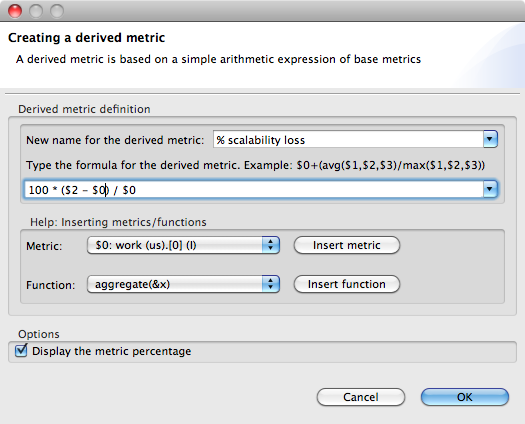
\includegraphics[width=0.8\textwidth]{fig/hpcviewer-dialog-derived-metric.png}}
\caption{Derived metric dialog box}
\label{fig:hpcviewer-derived-dialog-box}
\end{figure}

A derived metric can be created by clicking the \textbf{Derived metric} tool item in the navigation/control pane.
A derived metric window will then appear as shown in Figure~\ref{fig:hpcviewer-derived-dialog-box}.


The window has two main parts:
\begin{itemize}

\item \textbf{Derived metric definition}, which consists of:

\begin{itemize}

\item \textit{New name for the derived metric}.
  Supply a string that will be used as the column header for the derived metric.
  If you don't supply one, the metric will have no name.

\item \textit{Formula definition field}.
  In this field the user can define a formula with spreadsheet-like mathematical formula.
  This field is required to be filled.

\item \textit{Metric help}.
  This is used to help the user to find the \textit{ID} of a metric.
  For instance, in this snapshot, the metric \mysf{PAPI_TOT_CYC} has the ID \texttt{44}.
  By clicking the button \textbf{Insert metric}, the metric ID will be inserted in formula definition field.

\item \textit{Function help}.
  This help is to guide the user to insert functions in the formula definition field.
  Some functions require only one metric as the argument, but some can have two or more arguments.
  For instance, the function \texttt{avg()} which computes the average of some metrics, need to have two arguments.
\end{itemize}

\item \textbf{Advanced options}:
\begin{itemize}

\item \textit{Augment metric value display with a percentage relative to column total}.
  When this box is checked, each scope's derived metric value will be augmented with a percentage value, which for scope \textit{s} is computed as the 100 * (\textit{s}'s derived metric value) / (the derived metric value computed by applying the metric formula to the aggregate values of the input metrics) the entire execution).
  Such a computation can lead to nonsensical results for some derived metric formulae.
  For instance, if the derived metric is computed as a ratio of two other metrics, the aforementioned computation that compares the scope's ratio with the ratio for the entire program won't yield a meaningful result.
  To avoid a confusing metric display, think before you use this button to annotate a metric with its percent of total.

\item \textit{Default format}. This option will set the metric value with a scientific notation format which is the default format.

\item \textit{Display metric value as percent}. This option will set the metric value with percent format. For instance, if the metric has a value 12.345678, with this option, it's displayed as 12.34\%.

\item \textit{Custom format}. This option will set the metric value with your customized format. The format is equivalent to Java's Formatter class, or similar to C's printf format. For example, the format "\texttt{\%6.2f}" will display 6 digit floating-points with 2 digit precision.

\end{itemize}

\end{itemize}

Note that the entered formula and the metric name will be stored automatically.
One can then review again the formula (or metric name) by clicking the small triangle of the combo box (marked with a red circle).


% ===========================================================================
% ===========================================================================

\section{Plotting Graphs of Thread-level Metric Values}
\label{sec:hpcviewer:plots}

\begin{figure}[t]
\centering{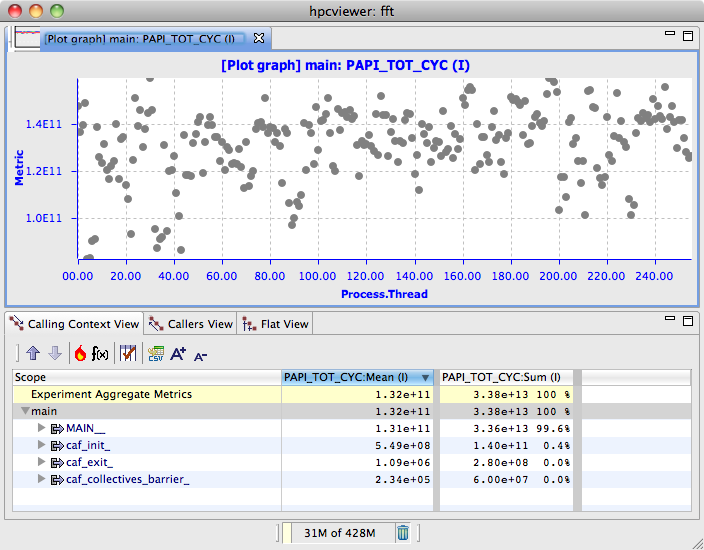
\includegraphics[width=0.8\textwidth]{fig/hpcviewer-view-rawmetrics.png}}
\caption{Plot graph view of main procedure in a Coarray Fortran application.}
\label{fig:hpcviewer-view-scatterplot}
\end{figure}


\HPCToolkit{} Experiment databases that have been generated by \hpcprofmpi{} (in contrast to \hpcprof{}) can be used by \hpcviewer{} to plot graphs of thread-level metric values.
This is particularly useful for quickly assessing load imbalance \emph{in context} across the several threads or processes of an execution.
Figure~\ref{fig:hpcviewer-view-scatterplot} shows \hpcviewer{} rendering such a plot.
The horizontal axis shows application processes, ordered by MPI rank.
The vertical axis shows metric values for each process.
Because \hpcviewer{} can generate scatter plots for any node in the Calling Context View, these graphs are calling-context sensitive.

To create a graph, first select a scope in the Calling Context View; in the Figure, the top-level procedure \texttt{main} is selected.
Then, right-click the selected scope to show the associated context menu.
(The menu begins with entries labeled `Zoom-in' and `Zoom-out.')
At the bottom of the context menu is a list of metrics that \hpcviewer{} can graph.
Each metric contains a sub-menu that lists the three different types of graphs \hpcviewer{} can plot:
\begin{itemize}
\item \textbf{Plot graph}.
  This standard graph plots metric values by their MPI rank (if available) and thread id (where ids are assigned by thread creation).

\item \textbf{Sorted plot graph}.
  This graph plots metric values in ascending order.

\item \textbf{Histogram graph}.
  This graph is a histogram of metric values.
  It divides the range of metric values into a small number of sub-ranges.
  The graph plots the frequency that a metric value falls into a particular sub-range.
\end{itemize}

Note that the viewers have the following notation for the ranks:
\begin{verbatim}
  <process_id> . <thread_id>
\end{verbatim}
Hence, if the ranks are 0.0, 0.1, \dots{} 31.0, 31.1 it means MPI process 0 has two threads: thread 0 and thread 1 (similarly with MPI process 31). 


Currently, it is only possible to generate scatter plots for metrics directly collected by \hpcrun{}, which excludes derived metrics created within \hpcviewer{}.



% ===========================================================================
% ===========================================================================

\section{For Convenience Sake}

In this section we describe some features of \hpcviewer{} that help improve productivity.

% ==========================================================
% ==========================================================

\subsection{Editor pane}

The editor pane is used to display \textit{a copy} of your program's source code or \HPCToolkit{}'s performance data in XML format; for this reason, it does not support editing of the pane's contents.
To edit your program, you should use your favorite editor to edit \textit{your} original copy of the source, not the one stored in \HPCToolkit{}'s performance database.
Thanks to built-in capabilities in Eclipse, \hpcviewer{} supports some useful shortcuts and customization:
\begin{itemize}
\item \textbf{Go to line}.
  To scroll the current source pane to a specific line number, \texttt{$<$ctrl$>$-l} (on Linux and Windows) or \texttt{$<$command$>$-l} (Mac) will bring up a dialog that enables you to enter the target line number.

\item \textbf{Find}.
  To search for a string in the current source pane, \texttt{$<$ctrl$>$-f} (Linux and Windows) or \texttt{$<$command$>$-f} (Mac) will bring up a find dialog that enables you to enter the target string.

\item \textbf{Font}.
  You can change the font used by \hpcviewer{} for the metric table using the Preferences dialog from the File menu.
  Once you've opened the Preferences dialog, select \textit{hpcviewer preferences} (the item at the bottom of the list in the column on the left side of the pane).
  The new font will take effect when you next launch \hpcviewer{}.

\item \textbf{Minimize/Maximize window}.
  Icons in the upper right corner of the window enable you to minimize (
\includegraphics[scale=.8]{fig/hpcviewer-button-minimize.png}) or maximize (
\includegraphics[scale=.8]{fig/hpcviewer-button-maximize.png}) the \hpcviewer{} window.
\end{itemize}


% ==========================================================
% ==========================================================

\subsection{Metric pane}
\label{sec:hpcviewer:metric-pane}

For the metric pane, \hpcviewer{} has some convenient features:
\begin{itemize}

\item \textbf{Maximizing a view}.
  To expand the source or metric pane to fill the window, one can double click on the tab with the view name.
  Double clicking again on the view name will restore the view back to its original size.

\item \textbf{Sorting the metric pane contents by a column's values}.
  First, select the column on which you wish to sort.
  If no triangle appears next to the metric, click again.
  A downward pointing triangle means that the rows in the metric pane are sorted in descending order according to the column's value.
  Additional clicks on the header of the selected column will toggle back and forth between ascending and descending.

\item \textbf{Changing column width}.
  To increase or decrease the width of a column, first put the cursor over the right or left border of the column's header field.
  The cursor will change into a vertical bar between a left and right arrow.
  Depress the mouse and drag the column border to the desired position.

\item \textbf{Changing column order}.
  If it would be more convenient to have columns displayed in a different order, they can be permuted as you wish.
  Depress and hold the mouse button over the header of column that you wish to move and drag the column right or left to its new position.

\item \textbf{Copying selected metrics into clipboard}.
  In order to copy selected lines of scopes/metrics, one can right click on the metric pane or navigation pane then select the menu \textbf{Copy}.
  The copied metrics can then be pasted into any text editor.

\item \textbf{Hiding or showing metric columns}.
  Sometimes, it may be more convenient to suppress the display of metrics that are not of current interest.
  When there are too many metrics to fit on the screen at once, it is often useful to suppress the display of some.
  The icon 
\includegraphics[scale=.7]{fig/hpcviewer-button-checkcolumns.png} above the metric pane will bring up the column selection dialog shown in Figure~\ref{fig:hpcviewer-hide-show-columns}.

\begin{figure}[t]
\centering{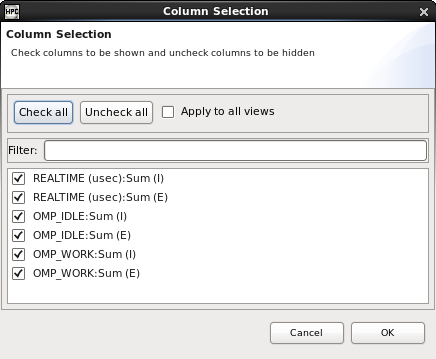
\includegraphics[width=0.8\textwidth]{fig/hpcviewer-dialog-checkcolumns.png}}
\caption{Hide/Show columns dialog box}
\label{fig:hpcviewer-hide-show-columns}
\end{figure}

The dialog box contains a list of metric columns sorted according to their order in \HPCToolkit{}'s performance database for the application.
Each metric column is prefixed by a check box to indicate if the metric should be \textit{displayed} (if checked) or \textit{hidden} (unchecked).
To display all metric columns, one can click the \textbf{Check all} button.
A click to \textbf{Uncheck all} will hide all the metric columns.

Finally, an option \textbf{Apply to all views} will set the configuration into all views when checked.
Otherwise, the configuration will be applied only on the current view.

\end{itemize}


% ===========================================================================
% ===========================================================================

\section{Menus}

\hpcviewer{} provides three main menus:

% ==========================================================
% ==========================================================

\subsection{File}
This menu includes several menu items for controlling basic viewer operations.
\begin{itemize}
\item \textbf{New window}
  Open a new \hpcviewer{} window that is independent from the existing one.

\item \textbf{Open database...}
  Load a performance database into the current \hpcviewer{} window. 
Currently \hpcviewer{} restricts maximum of five database open at a time. 
If you want to display more than five, you need to close an existing open database first.

\item \textbf{Close database...}
  Unloading one of more open performance database.

\item \textbf{Merge database CCT.../Merge database flat tree...}
  Merging two database that are currently in the viewer. If \hpcviewer{} has more than two
open database, then you need to choose which database you want to merge.
Currently \hpcviewer{} doesn't support storing a merged database into a file.

\item \textbf{Preferences...}
  Display the settings dialog box.

\item \textbf{Close window}
  Closing the current window. If there is only one window, then this menu will also exit \hpcviewer{} application.

\item \textbf{Exit}
  Quit the \hpcviewer{} application.

\end{itemize}

% ==========================================================
% ==========================================================

\subsection{View}
This menu is only visible if at least one database is loaded.
All actions in this menu are intended primarily for tool developer use. 
By default, the menu is hidden. Once you open a database, the menu is then shown.

\begin{itemize}
 \item \textbf{Show views}
 Display all the list of views (calling context views, callers view and flat view) for each database. If a view was closed, it will be suffixed by a "\texttt{*closed*}" sign.

 \item \textbf{Show metric properties}
 Display a list of metrics in a window. From this window, you can modify the name of the metric and in case of derived metrics, modify the formula as well as the format.

 \item \textbf{Debug}
 A special set of menus for advanced users. These menus are useful to debug \HPCToolkit{} and \hpcviewer{}. The menu consists of:

   \begin{itemize}
     \item \textbf{Show database raw's XML}
 	Enable one to request display of \HPCToolkit{}'s raw XML representation for performance data.

     \item \textbf{Show CCT label}
 	Display calling context ID for each node in the tree.

     \item \textbf{Show flat label}
 	Display static ID for each node in the tree.
  \end{itemize}

\end{itemize}
% ==========================================================
% ==========================================================

\subsection{Help}

This menu displays information about the viewer. The menu contains two items:
\begin{itemize}

\item \textbf{About}.
  Displays brief information about the viewer, including used plug-ins and error log.

\item \textbf{hpcviewer help}.
  This document.

\end{itemize}


% ===========================================================================
% ===========================================================================

\section{Limitations}

Some important \hpcviewer{} limitations are listed below:
\begin{itemize}

\item \textbf{Limited number of metrics}.
  With a large number of metric columns, \hpcviewer{}'s response time may become sluggish as this requires a large amount of memory.

%\item \textbf{Printing metrics}.
%  \hpcviewer{} does not currently support printing metric values.
%  However it is possible to export metrics into a file.

\end{itemize}
